\section{Analisis Popularitas Konferensi (\textit{Task} 2)}
\label{sec:hasil-t2}
Popularitas diukur dengan jumlah publikasi dan jumlah penulis unik (Subbab~\ref{sec:met-popularitas}). Nama lengkap konferensi yang disebut pada subbab ini diambil dari judul prosiding edisi utama terbaru pada \textit{dump} dan tercantum pada Tabel~\ref{tab:nama}.

\begin{table}[ht]
\caption{Nama lengkap konferensi pada sepuluh besar}
\label{tab:nama}
\small
\begin{tabularx}{\textwidth}{@{}lX@{}}
\toprule
\textbf{Singkatan} & \textbf{Nama lengkap} \\
\midrule
NeurIPS & \textit{Advances in Neural Information Processing Systems} \\
CVPR & \textit{IEEE/CVF Conference on Computer Vision and Pattern Recognition} \\
ICASSP & \textit{IEEE International Conference on Acoustics, Speech and Signal Processing} \\
HCI & \textit{HCI International} (\textit{International Conference on Human-Computer Interaction}) \\
IGARSS & \textit{IEEE International Geoscience and Remote Sensing Symposium} \\
AAAI & \textit{AAAI Conference on Artificial Intelligence} \\
CHI & \textit{ACM CHI Conference on Human Factors in Computing Systems} \\
EMNLP & \textit{Conference on Empirical Methods in Natural Language Processing} \\
EMBC & \textit{Annual International Conference of the IEEE Engineering in Medicine and Biology Society} \\
ICC & \textit{IEEE International Conference on Communications} \\
ICML & \textit{International Conference on Machine Learning} \\
IROS & \textit{IEEE/RSJ International Conference on Intelligent Robots and Systems} \\
\bottomrule
\end{tabularx}
\end{table}

\subsection{Sepuluh konferensi dengan publikasi terbanyak}
\label{sec:hasil-top-pub}
Tabel~\ref{tab:top-pub} dan Gambar~\ref{fig:top-pub} menunjukkan sepuluh konferensi dengan publikasi terbanyak. NeurIPS berada di peringkat pertama dengan 25.455 makalah (1,27\% dari seluruh \textit{dataset}), disusul CVPR (22.751) dan ICASSP (21.606).

\begin{table}[ht]
\caption{Sepuluh konferensi dengan publikasi terbanyak}
\label{tab:top-pub}
\small
\begin{tabular}{@{}rlrrrr@{}}
\toprule
\textbf{\#} & \textbf{Konferensi} & \textbf{Publikasi} & \textbf{Porsi} & \textbf{Peringkat penulis} & \textbf{Penulis unik} \\
\midrule
1 & NeurIPS & 25.455 & 1,27\% & 1 & 57.800 \\
2 & CVPR & 22.751 & 1,14\% & 2 & 47.664 \\
3 & ICASSP & 21.606 & 1,08\% & 4 & 42.057 \\
4 & HCI & 19.912 & 1,00\% & 6 & 37.884 \\
5 & IGARSS & 19.685 & 0,99\% & 7 & 35.229 \\
6 & AAAI & 19.274 & 0,97\% & 3 & 46.437 \\
7 & CHI & 14.832 & 0,74\% & 12 & 29.904 \\
8 & EMNLP & 14.813 & 0,74\% & 8 & 33.954 \\
9 & EMBC & 14.676 & 0,73\% & 5 & 39.318 \\
10 & ICC & 14.329 & 0,72\% & 19 & 26.626 \\
\bottomrule
\end{tabular}
\end{table}

\begin{figure}[ht]
\centering
\figtikz{fig-top10-publikasi}
\caption{Sepuluh konferensi dengan publikasi terbanyak}
\label{fig:top-pub}
\end{figure}

Sepuluh konferensi teratas menghasilkan 9,4\% seluruh publikasi. Daftar ini terbagi menjadi dua kelompok: enam konferensi pertama berada di atas 19.000 makalah, dan peringkat 7 sampai 10 berada rapat pada 14.300 sampai 14.800 makalah. Batas sepuluh besar sangat tipis karena ICC (14.329) hanya unggul 86 makalah dari GLOBECOM (14.243, peringkat 11). Daftar ini lintas bidang. Empat dari sepuluh tempat ditempati konferensi kecerdasan buatan dan pemrosesan bahasa alami (NeurIPS, CVPR, AAAI, EMNLP). Sisanya mencakup sinyal dan penginderaan jauh (ICASSP, IGARSS), interaksi manusia dan komputer (HCI, CHI), serta biomedis dan komunikasi (EMBC, ICC). Pengelompokan bidang ini adalah pengetahuan umum, bukan atribut dari data DBLP. Daftar ini bergantung pada keputusan menggabungkan \textit{workshop} ke konferensi induk (Subbab~\ref{sec:hasil-sensitivitas}).

\subsection{Sepuluh konferensi dengan penulis unik terbanyak}
\label{sec:hasil-top-author}
Tabel~\ref{tab:top-author} dan Gambar~\ref{fig:top-author} menunjukkan sepuluh konferensi dengan penulis unik terbanyak.

\begin{table}[ht]
\caption{Sepuluh konferensi dengan penulis unik terbanyak}
\label{tab:top-author}
\small
\begin{tabular}{@{}rlrrrr@{}}
\toprule
\textbf{\#} & \textbf{Konferensi} & \textbf{Penulis unik} & \textbf{Peringkat publikasi} & \textbf{Publikasi} & \textbf{Makalah per penulis} \\
\midrule
1 & NeurIPS & 57.800 & 1 & 25.455 & 2,18 \\
2 & CVPR & 47.664 & 2 & 22.751 & 2,50 \\
3 & AAAI & 46.437 & 6 & 19.274 & 1,83 \\
4 & ICASSP & 42.057 & 3 & 21.606 & 2,11 \\
5 & EMBC & 39.318 & 9 & 14.676 & 1,84 \\
6 & HCI & 37.884 & 4 & 19.912 & 1,83 \\
7 & IGARSS & 35.229 & 5 & 19.685 & 2,64 \\
8 & EMNLP & 33.954 & 8 & 14.813 & 2,16 \\
9 & ICML & 31.896 & 12 & 13.778 & 1,95 \\
10 & IROS & 31.249 & 14 & 12.851 & 1,83 \\
\bottomrule
\end{tabular}
\end{table}

\begin{figure}[ht]
\centering
\figtikz{fig-top10-author}
\caption{Sepuluh konferensi dengan penulis unik terbanyak}
\label{fig:top-author}
\end{figure}

Pada seluruh konferensi di daftar ini, penulis unik lebih banyak daripada jumlah makalah karena satu makalah ditulis beberapa orang. Ukuran makalah per penulis menunjukkan seberapa sering penulis kembali. IGARSS (2,64) dan CVPR (2,50) tertinggi, artinya rata-rata penulis menerbitkan dua sampai tiga makalah di sana. AAAI, HCI, IROS, dan EMBC terendah (sekitar 1,83), artinya komunitasnya lebih luas dan lebih banyak penulis yang hanya muncul satu kali. Dua konferensi baru muncul dibanding daftar publikasi, yaitu ICML dan IROS, sedangkan CHI dan ICC keluar dari daftar.

\subsection{Tren publikasi per tahun}
\label{sec:hasil-tren}
Tren seluruh \textit{dataset} telah dibahas pada Subbab~\ref{sec:hasil-tahun}. Gambar~\ref{fig:tren-top10} memperlihatkan tren sepuluh konferensi teratas dan Tabel~\ref{tab:pertumbuhan} merangkum pertumbuhannya dari 2015 ke 2024.

\begin{sidewaysfigure}
\centering
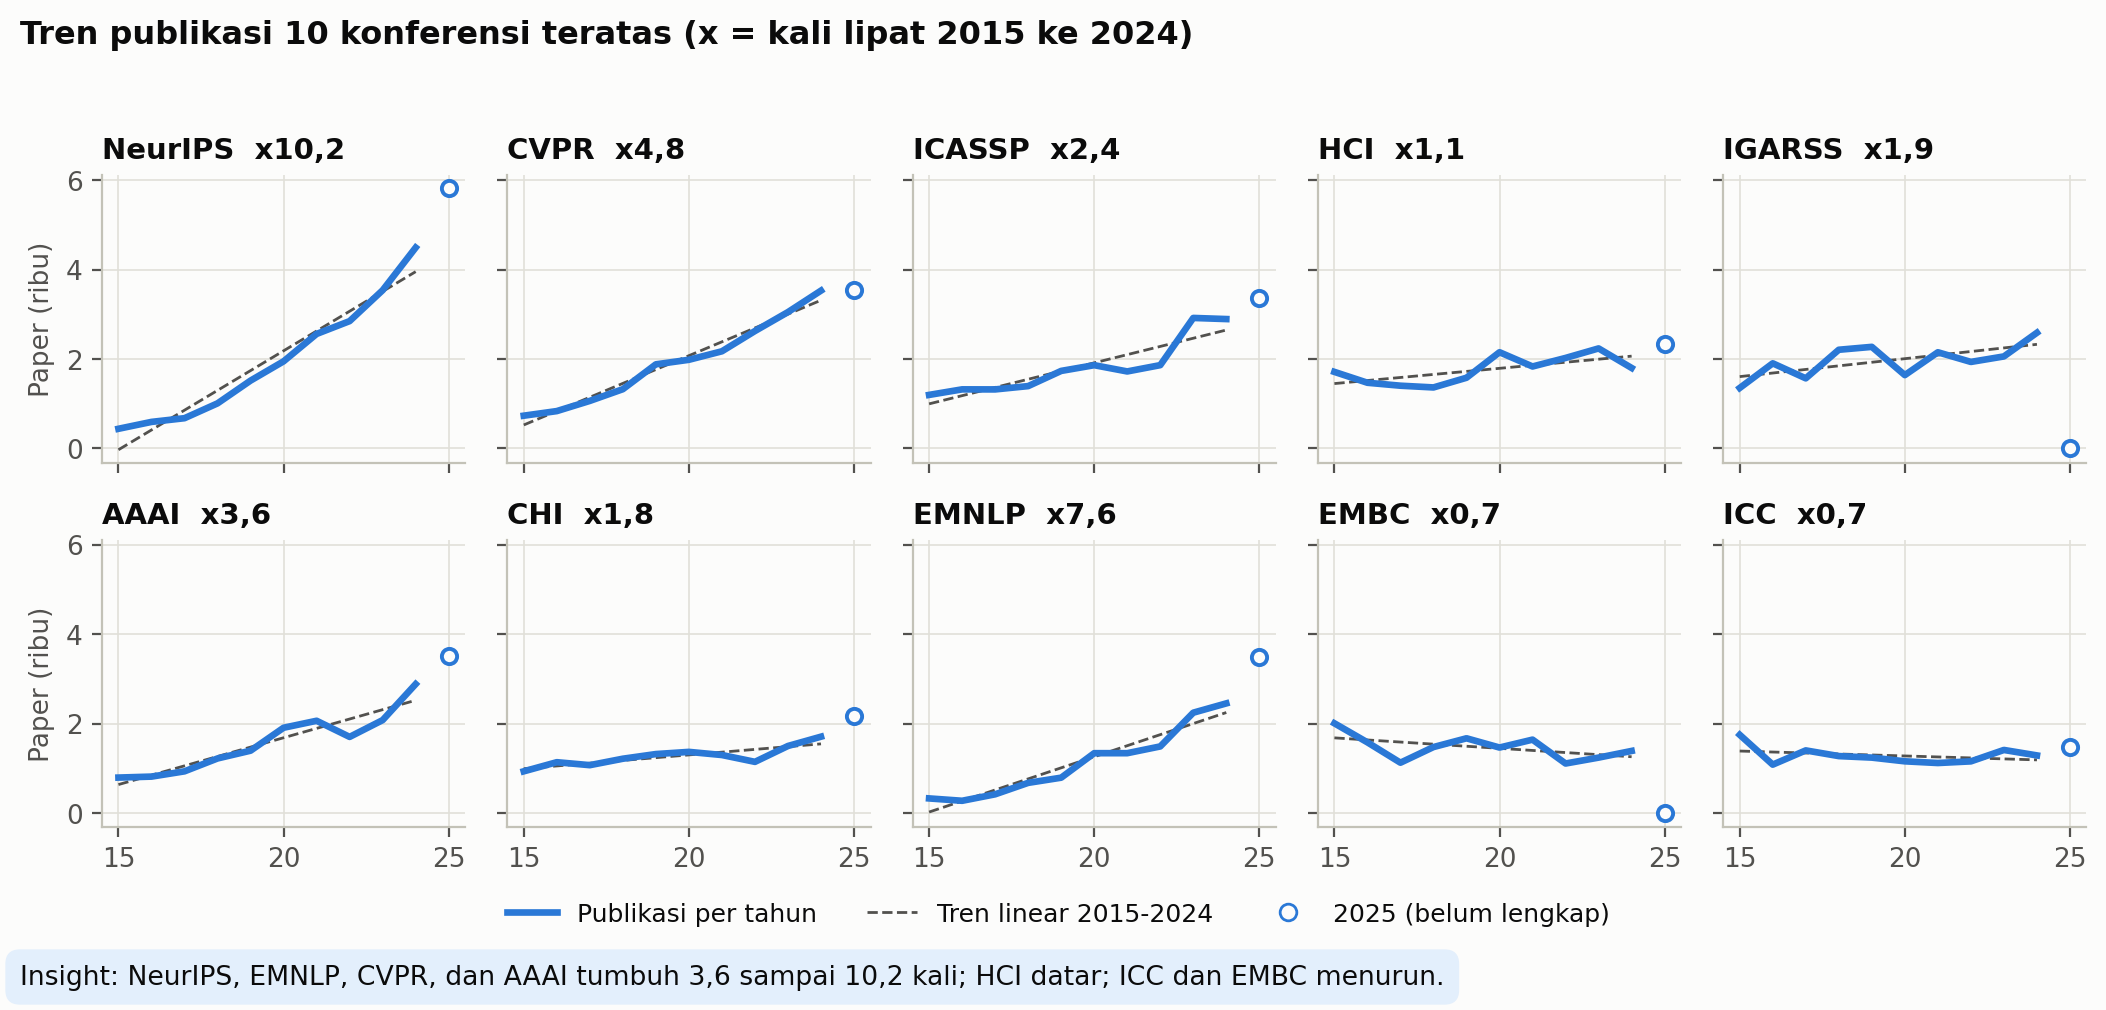
\includegraphics[width=\textheight,height=0.62\textwidth,keepaspectratio]{images/hasil/t2_tren_top10.png}
\caption{Tren publikasi per tahun pada sepuluh konferensi teratas (\textit{small multiples})}
\label{fig:tren-top10}
\end{sidewaysfigure}

\begin{table}[ht]
\caption{Pertumbuhan sepuluh konferensi teratas, 2015 ke 2024}
\label{tab:pertumbuhan}
\small
\begin{tabular}{@{}lrrrrr@{}}
\toprule
\textbf{Konferensi} & \textbf{2015} & \textbf{2024} & \textbf{Kali lipat} & \textbf{CAGR} & \textbf{2025} \\
\midrule
NeurIPS & 440 & 4.494 & 10,2 & $+$29,5\% & 5.823 \\
EMNLP & 324 & 2.450 & 7,6 & $+$25,2\% & 3.491 \\
CVPR & 733 & 3.531 & 4,8 & $+$19,1\% & 3.543 \\
AAAI & 790 & 2.882 & 3,6 & $+$15,5\% & 3.508 \\
ICASSP & 1.198 & 2.895 & 2,4 & $+$10,3\% & 3.370 \\
IGARSS & 1.353 & 2.589 & 1,9 & $+$7,5\% & 0 \\
CHI & 930 & 1.705 & 1,8 & $+$7,0\% & 2.168 \\
HCI & 1.713 & 1.801 & 1,1 & $+$0,6\% & 2.327 \\
ICC & 1.747 & 1.286 & 0,7 & $-$3,3\% & 1.479 \\
EMBC & 2.004 & 1.386 & 0,7 & $-$4,0\% & 0 \\
\bottomrule
\end{tabular}
\end{table}

Empat konferensi kecerdasan buatan dan pemrosesan bahasa alami (NeurIPS, EMNLP, CVPR, AAAI) tumbuh jauh di atas CAGR seluruh \textit{dataset} (3,2\%), yaitu 10,2, 7,6, 4,8, dan 3,6 kali lipat. HCI hampir datar, sedangkan ICC dan EMBC menurun. Gambar~\ref{fig:cagr} menampilkan laju pertumbuhan ini dibanding CAGR seluruh \textit{dataset}. Nilai 0 pada IGARSS dan EMBC untuk 2025 berarti belum terindeks, bukan berhenti, sebagaimana dijelaskan pada Subbab~\ref{sec:hasil-2025}.

\begin{figure}[ht]
\centering
\figtikz{fig-cagr-top10}
\caption{Laju pertumbuhan tahunan (CAGR) sepuluh konferensi teratas, 2015--2024}
\label{fig:cagr}
\end{figure}

Konsentrasi publikasi meningkat. Porsi sepuluh konferensi teratas terhadap seluruh publikasi sebesar 7,0\% pada 2015, turun ke titik terendah 6,5\% pada 2017, lalu naik menjadi 8,2\% (2019), 10,0\% (2021), dan 11,7\% (2024). Kenaikan berlangsung sejak 2017 sehingga bukan semata akibat data 2025 yang tidak lengkap. Gambar~\ref{fig:heatmap} memperluas pengamatan ke dua belas konferensi (delapan dengan indeks 2024 tertinggi dan empat terendah, dari dua puluh konferensi terbesar) dengan indeks terhadap rata-rata 2015--2017 konferensi itu sendiri (100 berarti sama dengan awal periode). Pada 2024, NeurIPS mencapai indeks 788, ICML 731, EMNLP 727, ACL 524, dan CVPR 402, sedangkan ICC (91), EMBC (88), dan IECON (86) berada di bawah level awal. ICLR dikeluarkan dari \textit{heatmap} karena DBLP tidak mencatatnya pada 2015 dan 2016 sehingga rata-rata awalnya tidak adil. Sejak 2017, ICLR tumbuh dari 309 menjadi 2.454 makalah pada 2024 sehingga termasuk konferensi dengan pertumbuhan tercepat.

\begin{sidewaysfigure}
\centering
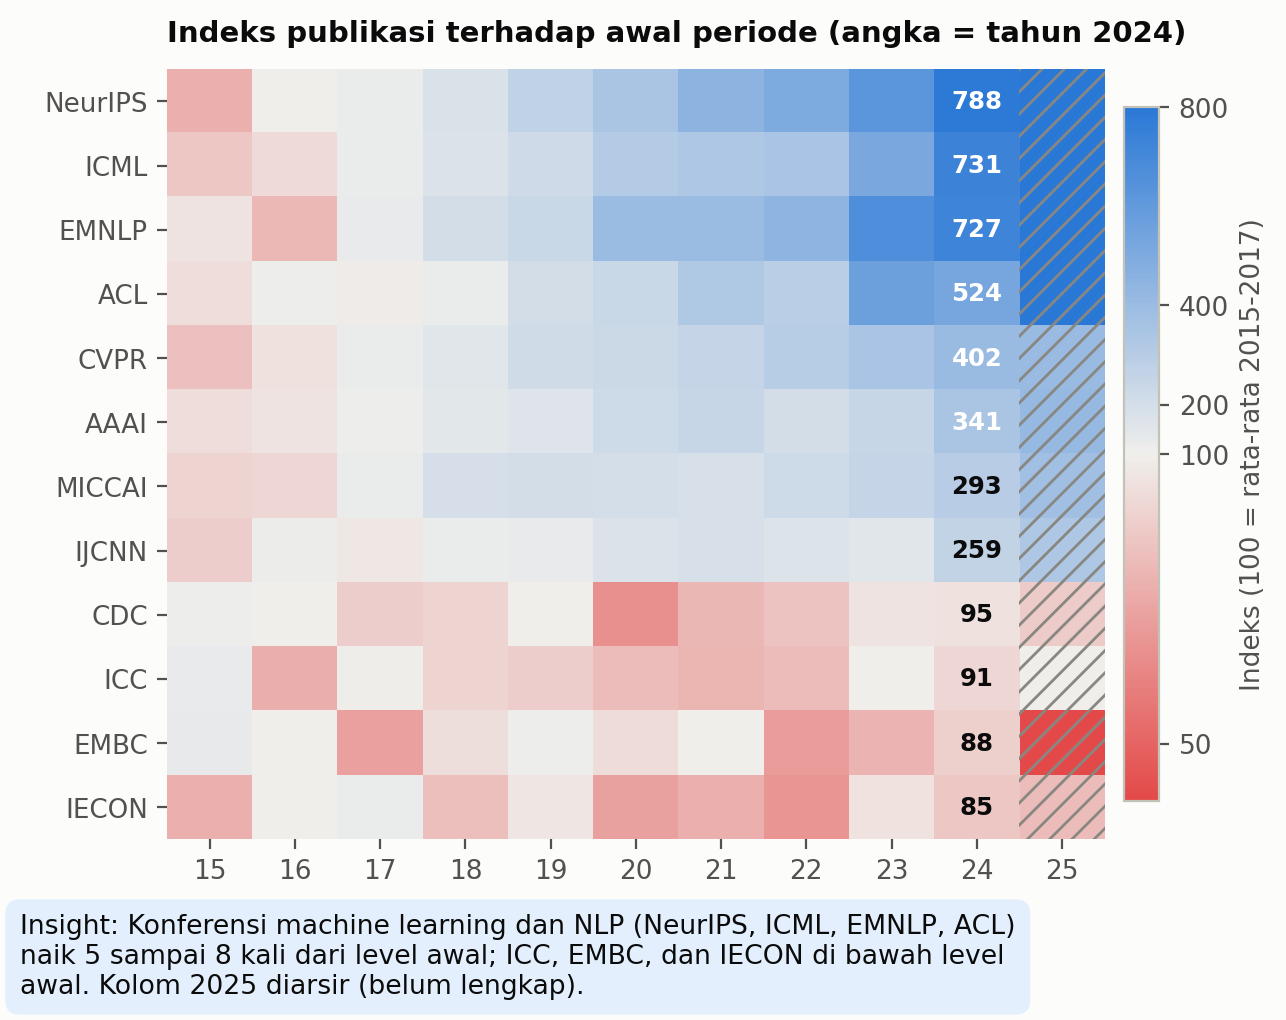
\includegraphics[width=\textheight,height=0.66\textwidth,keepaspectratio]{images/hasil/t2_heatmap_tren_top20.png}
\caption{Indeks publikasi dua belas konferensi terhadap rata-rata 2015--2017 (\textit{heatmap}); angka pada kolom 2024 adalah indeksnya}
\label{fig:heatmap}
\end{sidewaysfigure}

\subsection{Perbandingan peringkat publikasi dan penulis unik}
\label{sec:hasil-banding}
Tabel~\ref{tab:banding} dan Gambar~\ref{fig:slope} membandingkan peringkat kedua ukuran. Selisih adalah peringkat publikasi dikurangi peringkat penulis sehingga nilai positif berarti naik pada peringkat penulis unik.

\begin{table}[ht]
\caption{Perbandingan peringkat publikasi dan penulis unik}
\label{tab:banding}
\footnotesize
\setlength{\tabcolsep}{2.5pt}
\begin{tabular}{@{}lrrrrrl@{}}
\toprule
\textbf{Konferensi} & \textbf{Rank pub.} & \textbf{Rank penulis} & \textbf{Selisih} & \textbf{Penulis/ makalah} & \textbf{Makalah/ penulis} & \textbf{Masuk 10 besar} \\
\midrule
NeurIPS & 1 & 1 & 0 & 2,27 & 2,18 & keduanya \\
CVPR & 2 & 2 & 0 & 2,10 & 2,50 & keduanya \\
ICASSP & 3 & 4 & $-$1 & 1,95 & 2,11 & keduanya \\
HCI & 4 & 6 & $-$2 & 1,90 & 1,83 & keduanya \\
IGARSS & 5 & 7 & $-$2 & 1,79 & 2,64 & keduanya \\
AAAI & 6 & 3 & $+$3 & 2,41 & 1,83 & keduanya \\
CHI & 7 & 12 & $-$5 & 2,02 & 2,22 & publikasi saja \\
EMNLP & 8 & 8 & 0 & 2,29 & 2,16 & keduanya \\
EMBC & 9 & 5 & $+$4 & 2,68 & 1,84 & keduanya \\
ICC & 10 & 19 & $-$9 & 1,86 & 2,15 & publikasi saja \\
ICML & 12 & 9 & $+$3 & 2,31 & 1,95 & penulis saja \\
IROS & 14 & 10 & $+$4 & 2,43 & 1,83 & penulis saja \\
\bottomrule
\end{tabular}
\end{table}

\begin{figure}[ht]
\centering
\figtikz{fig-slope-peringkat}
\caption{Perubahan peringkat dari ukuran publikasi ke ukuran penulis unik}
\label{fig:slope}
\end{figure}

Kedua peringkat sangat selaras. Korelasi peringkat Spearman pada seluruh 4.373 \textit{venue} mencapai 0,987 (korelasi log-log 0,986), dan delapan dari sepuluh konferensi teratas sama. NeurIPS dan CVPR menempati posisi satu dan dua pada kedua ukuran, dan EMNLP tetap di posisi delapan. Perbedaan muncul di peringkat tengah. AAAI (6 ke 3) dan EMBC (9 ke 5) naik karena jumlah penulis unik per makalahnya tinggi (2,41 dan 2,68). CHI (7 ke 12) dan ICC (10 ke 19) turun, dan ICML serta IROS menggantikan keduanya pada sepuluh besar penulis unik. ICC mengalami penurunan terbesar (sembilan peringkat), dan 22,8\% makalahnya adalah makalah \textit{workshop} (Subbab~\ref{sec:hasil-sensitivitas}).

Gambar~\ref{fig:scatter} menunjukkan hubungan kedua ukuran pada seluruh \textit{venue}. Hampir semua konferensi berada di antara garis satu dan empat penulis unik per makalah dan mengelompok di sekitar dua. Jadi perbedaan peringkat berasal dari variasi rasio itu, bukan dari hubungan yang berbeda.

\begin{figure}[ht]
\centering
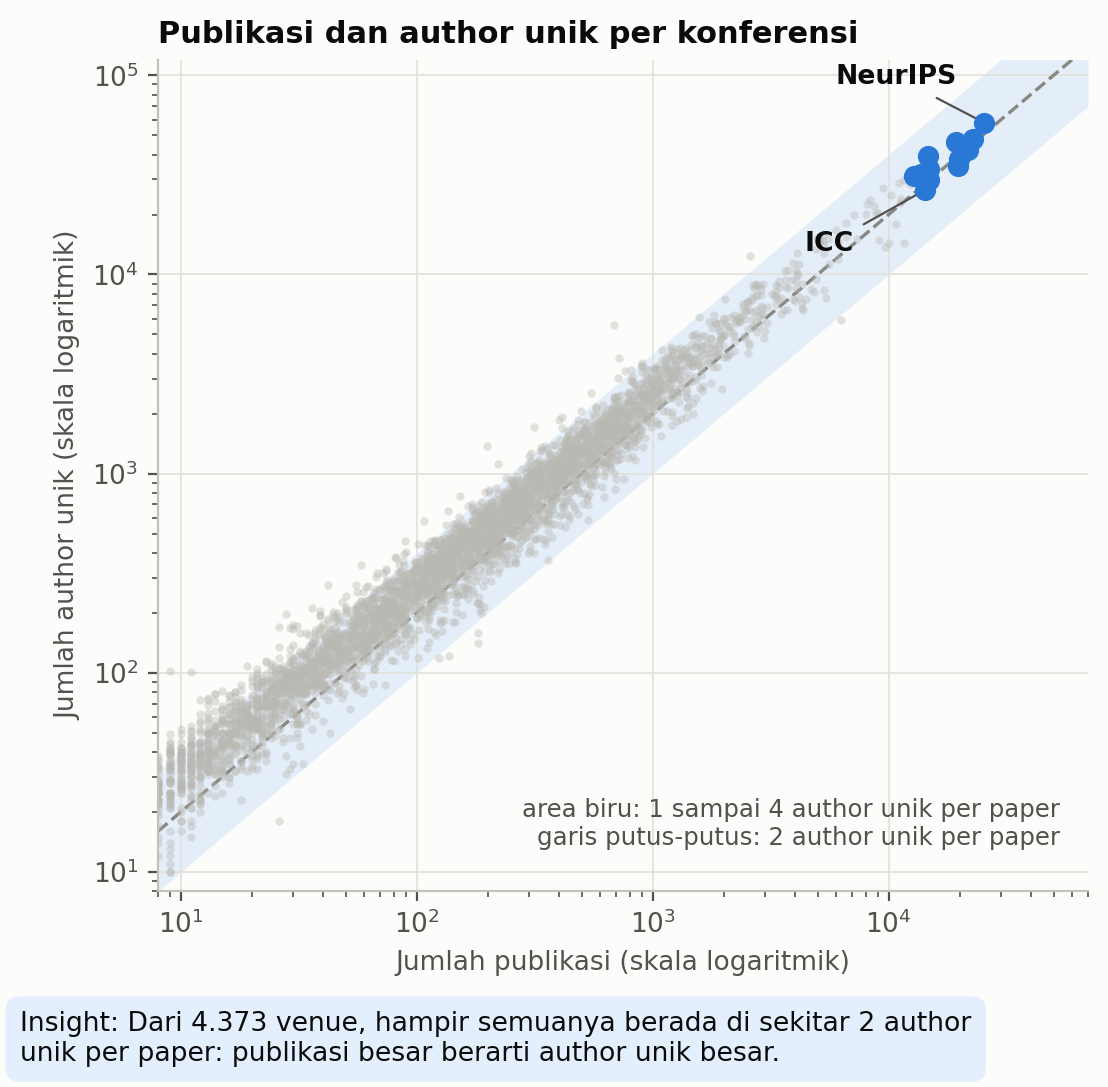
\includegraphics[width=0.9\textwidth]{images/hasil/t2_scatter_publikasi_author.png}
\caption{Publikasi dan penulis unik per konferensi (\textit{scatter} log-log); area biru menandai 1 sampai 4 penulis unik per makalah}
\label{fig:scatter}
\end{figure}

\subsection{Uji sensitivitas terhadap keputusan \textit{venue}}
\label{sec:hasil-sensitivitas}
Karena \textit{venue} diambil dari \textit{key}, \textit{workshop} dan acara pendamping ikut terhitung sebagai konferensi induknya. Untuk menguji apakah kesimpulan bergantung pada keputusan itu, peringkat dihitung ulang tanpa acara satelit yang dikenali dari kata kunci \textit{booktitle} (Subbab~\ref{sec:satelit}). Pengenalan ini adalah pendekatan, bukan definisi pasti. Hasilnya ditunjukkan pada Tabel~\ref{tab:sensitivitas}.

\begin{table}[ht]
\caption{Peringkat publikasi dengan dan tanpa acara satelit}
\label{tab:sensitivitas}
\small
\begin{tabular}{@{}lrrrrr@{}}
\toprule
\textbf{Konferensi} & \textbf{Seluruh \textit{key}} & \textbf{Tanpa satelit} & \textbf{Porsi satelit} & \textbf{Rank awal} & \textbf{Rank baru} \\
\midrule
NeurIPS & 25.455 & 25.178 & 1,1\% & 1 & 1 \\
CVPR & 22.751 & 17.422 & 23,4\% & 2 & 6 \\
ICASSP & 21.606 & 21.125 & 2,2\% & 3 & 2 \\
HCI & 19.912 & 19.912 & 0,0\% & 4 & 3 \\
IGARSS & 19.685 & 19.685 & 0,0\% & 5 & 4 \\
AAAI & 19.274 & 18.435 & 4,4\% & 6 & 5 \\
CHI & 14.832 & 8.303 & 44,0\% & 7 & 29 \\
EMNLP & 14.813 & 14.067 & 5,0\% & 8 & 8 \\
EMBC & 14.676 & 14.676 & 0,0\% & 9 & 7 \\
ICC & 14.329 & 11.064 & 22,8\% & 10 & 18 \\
ICML & 13.778 & 13.701 & 0,6\% & 12 & 9 \\
\bottomrule
\end{tabular}
\end{table}

Peringkat teratas relatif kuat. Delapan dari sepuluh konferensi teratas tetap sama dan NeurIPS tetap nomor satu, sedangkan ICML dan IROS masuk sepuluh besar dan CHI serta ICC keluar. Konferensi dengan banyak acara pendamping paling terpengaruh: CVPR (2 ke 6, karena \textit{CVPR Workshops}), ICC (10 ke 18, karena \textit{ICC Workshops}), dan CHI (7 ke 29, karena \textit{CHI Extended Abstracts} yang mencapai 44\%). Pernyataan bahwa CVPR adalah konferensi paling populer kedua bergantung pada definisi. Pernyataan itu benar jika \textit{workshop} dihitung bagian konferensi, sesuai pengelompokan DBLP, dan tidak benar jika hanya acara utama yang dihitung. Jawaban \textit{Task} 2 memakai definisi berbasis \textit{key}.

\subsection{Jawaban pertanyaan \textit{Task} 2}
\label{sec:jawab-t2}
\textbf{Konferensi paling populer berdasarkan jumlah publikasi.} Dari 1.997.244 publikasi pada 2015--2025, NeurIPS memiliki publikasi terbanyak dengan 25.455 makalah (1,27\% dari seluruh \textit{dataset}), disusul CVPR (22.751) dan ICASSP (21.606). NeurIPS tetap berada di peringkat pertama ketika \textit{workshop} dan acara satelit dikeluarkan.

\textbf{Hubungan publikasi dan penulis unik.} Konferensi dengan publikasi terbanyak juga memiliki penulis unik terbanyak untuk peringkat teratas. NeurIPS menempati peringkat pertama pada kedua ukuran (25.455 makalah dan 57.800 penulis unik), dan CVPR peringkat kedua pada keduanya. Delapan dari sepuluh konferensi teratas sama, dan korelasi peringkat Spearman pada 4.373 konferensi mencapai 0,987. Perbedaan terjadi pada peringkat tengah. AAAI dan EMBC lebih tinggi pada penulis unik karena menarik lebih banyak penulis berbeda per makalah, sedangkan ICC berada di peringkat 10 pada publikasi tetapi hanya peringkat 19 pada penulis unik.

\textbf{Perubahan aktivitas selama periode pengamatan.} Jumlah publikasi tumbuh 32,7\% dari 160.800 (2015) menjadi 213.328 (2024), setara CAGR 3,2\% per tahun, dengan penurunan 8,8\% pada 2020. Pertumbuhan sangat tidak merata. NeurIPS, EMNLP, CVPR, dan AAAI tumbuh 10,2, 7,6, 4,8, dan 3,6 kali, sedangkan HCI hampir datar serta ICC dan EMBC menurun. Akibatnya porsi sepuluh konferensi teratas naik dari 7,0\% pada 2015 menjadi 11,7\% pada 2024. Data 2025 tidak dipakai untuk menyimpulkan tren karena sebagian konferensi dua tahunan tidak diadakan pada tahun tersebut dan sebagian konferensi tahunan belum terindeks.
